\section{Digital Signal Processing (DSP) - Session
2}\label{digital-signal-processing-dsp---session-2}

\subsection{I. Introduction}\label{i.-introduction}

\subsubsection{1. The Concept of Frequency in Continuous-Time and
Discrete-Time
Signals}\label{the-concept-of-frequency-in-continuous-time-and-discrete-time-signals}

\paragraph{1.1. Continuous-Time Sinusoidal
Signals}\label{continuous-time-sinusoidal-signals}

A simple harmonic oscillation is mathematically described by a
continuous-time sinusoidal signal. A continuous-time sinusoid is
completely characterized by three parameters: amplitude (\(A\)),
frequency (\(\Omega\) or \(F\)), and phase (\(\theta\)).

\textbf{General Expression (Radians):}

\[  
x(t)=A\cos(\Omega t+\theta),  
\qquad -\infty<t<\infty  
\]

where

\begin{itemize}
\tightlist
\item
  \(A\) is the amplitude.
\item
  \(\Omega\) is the angular frequency in \textbf{radians per second
  (rad/s)}.
\item
  \(t\) is time in \textbf{seconds}.
\item
  \(\theta\) is the phase in \textbf{radians}.
\end{itemize}

\textbf{Frequency Relation:}

\[  
\Omega = 2\pi F  
\]

where

\begin{itemize}
\tightlist
\item
  \(F\) is the frequency in \textbf{cycles per second (Hz)}.
\end{itemize}

\textbf{General Expression (Hertz):}

\[  
x(t)=A\cos(2\pi Ft+\theta),  
\qquad -\infty<t<\infty  
\]

\textbf{Periodicity:} For every fixed value of \(F\), the signal is
periodic.

\[  
x(t+T)=x(t)  
\]

The fundamental period is \(T=1/F\).

\textbf{Uniqueness:} Continuous-time sinusoidal signals with distinct
frequencies are distinct.

\textbf{Rate of Oscillation:} Increasing \(F\) increases the rate of
oscillation (more cycles within a given time interval). Since time is
continuous, the frequency \(F\) can increase without bound.

\textbf{Complex Exponential Form and Phasors:}

\[  
x(t)
=
Ae^{j(\Omega t+\theta)}  
\]

Sinusoidal signals are closely related to complex exponential signals
through \textbf{Euler's identity}:

\[  
e^{j\phi}
=
\cos\phi  
+  
j\sin\phi  
\]

A real sinusoidal signal can be expressed as the sum of two
equal-amplitude complex-conjugate exponentials:

\[  
x(t)
=
A\cos(\Omega t+\theta)
=
\frac{A}{2}e^{j(\Omega t+\theta)}  
+  
\frac{A}{2}e^{-j(\Omega t+\theta)}  
\]

\textbf{Frequency Range:} Although physical frequency is nonnegative,
both positive and negative frequencies are used for mathematical
convenience.

\[  
-\infty<F<\infty  
\]

\paragraph{1.2. Discrete-Time Sinusoidal
Signals}\label{discrete-time-sinusoidal-signals}

A discrete-time sinusoidal signal is a sequence of numbers derived from
a function of an integer variable \(n\).

\textbf{General Expression (Radians):}

\[  
x[n]=A\cos(\omega n+\theta),  
\qquad -\infty<n<\infty  
\]

where

\begin{itemize}
\tightlist
\item
  \(A\) is the amplitude.
\item
  \(\omega\) is the angular frequency in \textbf{radians per sample}.
\item
  \(n\) is the \textbf{sample index} (an integer).
\item
  \(\theta\) is the phase in \textbf{radians}.
\end{itemize}

\textbf{Frequency Relation:}

\[  
\omega=2\pi f  
\]

where

\begin{itemize}
\tightlist
\item
  \(f\) is the frequency in \textbf{cycles per sample}.
\end{itemize}

\textbf{General Expression (Cycles):}

\[  
x[n]=A\cos(2\pi fn+\theta),  
\qquad -\infty<n<\infty  
\]

\textbf{Periodicity:} A discrete-time sinusoid is periodic \textbf{only
if} its normalized frequency \(f\) is a \textbf{rational number}. A
signal is periodic with period \(N\) (\(N>0\)) if

\[  
x[n+N]=x[n]
\]

This requires \(f_0=k/N\) where \(k\) and \(N\) are integers. The
fundamental period is obtained by expressing \(f_0\) as a reduced
fraction \(k/N\), where \(k\) and \(N\) are relatively prime.

\textbf{Uniqueness and Aliasing:} Discrete-time sinusoids whose
frequencies differ by an integer multiple of \(2\pi\) are identical.

\[  
\cos\!\left[(\omega_0+2\pi)n+\theta\right]
=
\cos\!\left(\omega_0n+2\pi n+\theta\right)
=
\cos(\omega_0n+\theta)  
\]

Therefore, every frequency outside the principal interval is an
\textbf{alias} of a frequency inside it.

The unique frequency ranges are commonly chosen as
\(-\pi\le\omega\le\pi\) or equivalently \(-\frac12\le f\le\frac12\).

\textbf{Highest Rate of Oscillation:} The highest rate of oscillation
occurs at \(\omega=\pi\) or \(\omega=-\pi\). This corresponds to
\(f=\frac12\) or \(f=-\frac12\).

Observations:

\begin{itemize}
\tightlist
\item
  Increasing \(\omega\) from \(0\) to \(\pi\) increases the rate of
  oscillation.
\item
  Increasing \(\omega\) from \(\pi\) to \(2\pi\) decreases the apparent
  rate of oscillation because of aliasing.
\end{itemize}

\textbf{Complex Exponential Form:} Using Euler's identity, a
discrete-time sinusoid can be expressed as the sum of two
complex-conjugate exponentials:

\[  
x[n]
=
A\cos(\omega n+\theta)
=
\frac{A}{2}e^{j(\omega n+\theta)}  
+  
\frac{A}{2}e^{-j(\omega n+\theta)}  
\]

\textbf{Frequency Range:} Unlike continuous-time sinusoids,
discrete-time frequencies repeat every \(2\pi\). The frequency axis is
periodic with period \(2\pi\).

Two commonly used principal frequency intervals are
\(0\le\omega\le2\pi\) and \(-\pi\le\omega\le\pi\).

\subsubsection{2. Analog-to-Digital Conversion
(ADC)}\label{analog-to-digital-conversion-adc}

\paragraph{2.1. Basic parts}\label{basic-parts}

\begin{itemize}
\tightlist
\item
  Goal: convert a continuous-time, continuous-amplitude signal into a
  discrete-time, discrete-amplitude sequence.
\item
  Typical chain: \textbf{anti-aliasing filter} → \textbf{sampling} →
  \textbf{quantization} → \textbf{encoding}.
\end{itemize}

\begin{enumerate}
\def\labelenumi{\arabic{enumi}.}
\tightlist
\item
  Sampling

  \begin{itemize}
  \item
    Sample at rate \(f_s\) samples/second (sampling period
    \(T_s=1/f_s\)):

    \[  
      x[n]=x_a(nT_s)  
      \]
  \item
    Sampling a signal multiplies it by an impulse train in time, which
    creates \textbf{spectral replicas} in frequency.
  \item
    In discrete-time, the corresponding digital frequency is
    \(\omega = 2\pi f/f_s\).
  \end{itemize}
\item
  Quantization

  \begin{itemize}
  \item
    Rounds each sample to the nearest value on a finite set of amplitude
    levels.
  \item
    Quantization step size (uniform quantizer):

    \[  
      \Delta = \frac{V_{\max}-V_{\min}}{2^B}  
      \]

    where \(B\) is number of bits.
  \item
    Quantization error:

    \[  
      e_q[n]=x[n]-x_q[n].  
      \]
  \end{itemize}
\item
  Encoding

  \begin{itemize}
  \tightlist
  \item
    Maps each quantized level to a binary word of length \(B\).
  \item
    Bit rate (for one channel): \(R = B\,f_s\) bits/second.
  \end{itemize}
\end{enumerate}

\paragraph{2.2. Nyquist--Shannon sampling theorem \&
Aliasing}\label{nyquistshannon-sampling-theorem-aliasing}

\begin{itemize}
\tightlist
\item
  If a continuous-time signal is bandlimited to \(|f|\le B\) Hz, then
  perfect reconstruction is possible when \(f_s \ge 2B\) (Nyquist rate).
\item
  If \(f_s < 2B\), spectral replicas overlap → \textbf{aliasing},
  meaning high-frequency content folds into lower frequencies.
\item
  Practical note: because real signals are not perfectly bandlimited, we
  usually use an \textbf{anti-aliasing low-pass filter} before sampling.
\end{itemize}

\paragraph{2.3. Signal-to-quantization noise ratio
(SQNR)}\label{signal-to-quantization-noise-ratio-sqnr}

\begin{itemize}
\item
  SQNR measures the ratio of signal power to quantization-noise power:

  \[  
    \text{SQNR}=\frac{P_{\text{signal}}}{P_{\text{quant}}}=\frac{3}{2}\cdot 2^{2B}  
    \]
\item
  SQNR is also often expressed in decibels (dB):
\end{itemize}

\[  
\text{SQNR}_{\text{dB}}=10\log_{10}(\text{SQNR}) \approx 1.76 + 6.02B  
\]

\emph{Tip (logarithmic scale / dB):} Use a log scale when quantities
span many orders of magnitude (very large or very small).

\begin{itemize}
\tightlist
\item
  \textbf{Power ratio (dB):}
  \(P_{\mathrm{dB}} = 10\log_{10}\!\left(\frac{P_2}{P_1}\right)\)
\item
  \textbf{Amplitude ratio (dB):}
  \(A_{\mathrm{dB}} = 20\log_{10}\!\left(\frac{A_2}{A_1}\right)\)
  (because \(P \propto A^2\))
\end{itemize}

\subsection{II. Discrete-Time Signals}\label{ii.-discrete-time-signals}

\subsubsection{1. Representations}\label{representations}

Discrete-time signals \(x[n]\) are defined only for integer values of
the independent variable \(n \in \mathbb{Z}\). They can be represented
in four standard forms:

\begin{itemize}
\tightlist
\item
  \textbf{Graphical:} A stem plot displaying sample values (amplitudes)
  as discrete vertical lines plotted against integer indices \(n\).
\item
  \textbf{Functional:} A piecewise or closed-form mathematical
  expression defining \(x[n]\) for all \(n\).

  \begin{itemize}
  \tightlist
  \item
    \emph{Example:} \(x[n] = 2^n u[n]\)
  \end{itemize}
\item
  \textbf{Tabular:} A table listing discrete sample values directly
  corresponding to specific values of \(n\).
\item
  \textbf{Sequence (Vector):} An ordered set of numbers enclosed in
  brackets, where an arrow or bold term indicates the sample index
  \(n = 0\).

  \begin{itemize}
  \tightlist
  \item
    \emph{Example:}
    \(x[n] = \{\dots, 0, \underset{\uparrow}{2}, 1, 3, 0, \dots\}\) (the
    arrow highlights \(x[0] = 2\)).
  \end{itemize}
\end{itemize}

\subsubsection{2. Some Elementary Discrete-Time
Signals}\label{some-elementary-discrete-time-signals}

\paragraph{2.1. Unit Sample Signal (Impulse
Signal)}\label{unit-sample-signal-impulse-signal}

Defines a single isolated spike of unit amplitude at \(n = 0\):

\[  
\delta[n] = \begin{cases} 1, & \text{if } n = 0 \\ 0, & \text{if } n \neq 0 \end{cases}  
\]

\paragraph{2.2. Unit Step Signal}\label{unit-step-signal}

Represents a signal that gets activated at \(n = 0\) with constant unit
amplitude:

\[  
u[n] = \begin{cases} 1, & \text{if } n \ge 0 \\ 0, & \text{if } n < 0 \end{cases}  
\]

\begin{itemize}
\tightlist
\item
  \emph{Relationship to Impulse:}
\end{itemize}

\[
u[n] = \sum_{k=-\infty}^{n} \delta[k] = \sum_{k=0}^{\infty} \delta[n-k]
\]

\paragraph{2,3. Unit Ramp Signal}\label{unit-ramp-signal}

A signal that grows linearly with sample index \(n\) for non-negative
time:

\[  
r[n] = \begin{cases} n, & \text{if } n \ge 0 \\ 0, & \text{if } n < 0 \end{cases}  
\]

\begin{itemize}
\tightlist
\item
  \emph{Relationship to Unit Step:}
\end{itemize}

\[
r[n] = n \cdot u[n]
\]

\paragraph{2.4. Exponential Signals}\label{exponential-signals}

General discrete-time exponential signals take the form \(x[n] = a^n\):

\begin{itemize}
\tightlist
\item
  \textbf{Real Exponential (\(x[n] = a^n\), where
  \(a \in \mathbb{R}\)):}

  \begin{itemize}
  \tightlist
  \item
    \(|a| > 1\): Growing exponential.
  \item
    \(|a| < 1\): Decaying exponential.
  \item
    \(a < 0\): Alternating signs between positive and negative samples.
  \end{itemize}
\item
  \textbf{Complex Exponential (\(x[n] = e^{j\omega_0 n}\)):}

  \begin{itemize}
  \tightlist
  \item
    Expressed via Euler's formula:
    \(e^{j\omega_0 n} = \cos(\omega_0 n) + j \sin(\omega_0 n)\).
  \item
    Unlike continuous complex exponentials, discrete complex
    exponentials are \textbf{periodic only if} \(\frac{\omega_0}{2\pi}\)
    is a rational number.
  \end{itemize}
\end{itemize}

\emph{Example:} Sketch the graph of this signal:

\[  
x[n]=u[n-2]-u[n-5]  
\]

\begin{Shaded}
\begin{Highlighting}[]
\ImportTok{import}\NormalTok{ numpy }\ImportTok{as}\NormalTok{ np}
\ImportTok{import}\NormalTok{ matplotlib.pyplot }\ImportTok{as}\NormalTok{ plt}

\CommentTok{\# Define the index range}
\NormalTok{n }\OperatorTok{=}\NormalTok{ np.arange(}\OperatorTok{{-}}\DecValTok{2}\NormalTok{, }\DecValTok{9}\NormalTok{)}

\CommentTok{\# Define step function u[n]}
\KeywordTok{def}\NormalTok{ u(n):}
    \ControlFlowTok{return}\NormalTok{ np.where(n }\OperatorTok{\textgreater{}=} \DecValTok{0}\NormalTok{, }\DecValTok{1}\NormalTok{, }\DecValTok{0}\NormalTok{)}

\CommentTok{\# Signals}
\NormalTok{u\_n2 }\OperatorTok{=}\NormalTok{ u(n }\OperatorTok{{-}} \DecValTok{2}\NormalTok{)}
\NormalTok{u\_n5 }\OperatorTok{=}\NormalTok{ u(n }\OperatorTok{{-}} \DecValTok{5}\NormalTok{)}
\NormalTok{x\_n }\OperatorTok{=}\NormalTok{ u\_n2 }\OperatorTok{{-}}\NormalTok{ u\_n5}

\CommentTok{\# Plot step{-}by{-}step}
\NormalTok{fig, axes }\OperatorTok{=}\NormalTok{ plt.subplots(}\DecValTok{3}\NormalTok{, }\DecValTok{1}\NormalTok{, figsize}\OperatorTok{=}\NormalTok{(}\DecValTok{8}\NormalTok{, }\DecValTok{7}\NormalTok{), sharex}\OperatorTok{=}\VariableTok{True}\NormalTok{)}

\CommentTok{\# Plot 1: u[n{-}2]}
\NormalTok{axes[}\DecValTok{0}\NormalTok{].stem(n, u\_n2, basefmt}\OperatorTok{=}\StringTok{"C0{-}"}\NormalTok{)}
\NormalTok{axes[}\DecValTok{0}\NormalTok{].set\_ylabel(}\StringTok{\textquotesingle{}$u[n{-}2]$\textquotesingle{}}\NormalTok{, fontsize}\OperatorTok{=}\DecValTok{12}\NormalTok{)}
\NormalTok{axes[}\DecValTok{0}\NormalTok{].set\_title(}\StringTok{\textquotesingle{}Step 1: First Shifted Unit Step $u[n{-}2]$\textquotesingle{}}\NormalTok{, fontsize}\OperatorTok{=}\DecValTok{12}\NormalTok{)}
\NormalTok{axes[}\DecValTok{0}\NormalTok{].set\_yticks([}\DecValTok{0}\NormalTok{, }\DecValTok{1}\NormalTok{])}
\NormalTok{axes[}\DecValTok{0}\NormalTok{].grid(}\VariableTok{True}\NormalTok{, linestyle}\OperatorTok{=}\StringTok{\textquotesingle{}{-}{-}\textquotesingle{}}\NormalTok{, alpha}\OperatorTok{=}\FloatTok{0.6}\NormalTok{)}

\CommentTok{\# Plot 2: u[n{-}5]}
\NormalTok{axes[}\DecValTok{1}\NormalTok{].stem(n, u\_n5, basefmt}\OperatorTok{=}\StringTok{"C0{-}"}\NormalTok{)}
\NormalTok{axes[}\DecValTok{1}\NormalTok{].set\_ylabel(}\StringTok{\textquotesingle{}$u[n{-}5]$\textquotesingle{}}\NormalTok{, fontsize}\OperatorTok{=}\DecValTok{12}\NormalTok{)}
\NormalTok{axes[}\DecValTok{1}\NormalTok{].set\_title(}\StringTok{\textquotesingle{}Step 2: Second Shifted Unit Step $u[n{-}5]$\textquotesingle{}}\NormalTok{, fontsize}\OperatorTok{=}\DecValTok{12}\NormalTok{)}
\NormalTok{axes[}\DecValTok{1}\NormalTok{].set\_yticks([}\DecValTok{0}\NormalTok{, }\DecValTok{1}\NormalTok{])}
\NormalTok{axes[}\DecValTok{1}\NormalTok{].grid(}\VariableTok{True}\NormalTok{, linestyle}\OperatorTok{=}\StringTok{\textquotesingle{}{-}{-}\textquotesingle{}}\NormalTok{, alpha}\OperatorTok{=}\FloatTok{0.6}\NormalTok{)}

\CommentTok{\# Plot 3: x[n] = u[n{-}2] {-} u[n{-}5]}
\NormalTok{axes[}\DecValTok{2}\NormalTok{].stem(n, x\_n, basefmt}\OperatorTok{=}\StringTok{"C0{-}"}\NormalTok{)}
\NormalTok{axes[}\DecValTok{2}\NormalTok{].set\_ylabel(}\StringTok{\textquotesingle{}$x[n]$\textquotesingle{}}\NormalTok{, fontsize}\OperatorTok{=}\DecValTok{12}\NormalTok{)}
\NormalTok{axes[}\DecValTok{2}\NormalTok{].set\_xlabel(}\StringTok{\textquotesingle{}Sample Index $n$\textquotesingle{}}\NormalTok{, fontsize}\OperatorTok{=}\DecValTok{12}\NormalTok{)}
\NormalTok{axes[}\DecValTok{2}\NormalTok{].set\_title(}\StringTok{\textquotesingle{}Step 3: Resulting Signal $x[n] = u[n{-}2] {-} u[n{-}5]$\textquotesingle{}}\NormalTok{, fontsize}\OperatorTok{=}\DecValTok{12}\NormalTok{)}
\NormalTok{axes[}\DecValTok{2}\NormalTok{].set\_yticks([}\DecValTok{0}\NormalTok{, }\DecValTok{1}\NormalTok{])}
\NormalTok{axes[}\DecValTok{2}\NormalTok{].grid(}\VariableTok{True}\NormalTok{, linestyle}\OperatorTok{=}\StringTok{\textquotesingle{}{-}{-}\textquotesingle{}}\NormalTok{, alpha}\OperatorTok{=}\FloatTok{0.6}\NormalTok{)}

\NormalTok{plt.tight\_layout()}
\NormalTok{plt.savefig(}\StringTok{"signal\_visualization.png"}\NormalTok{, dpi}\OperatorTok{=}\DecValTok{300}\NormalTok{)}
\NormalTok{plt.show()}

\BuiltInTok{print}\NormalTok{(}\StringTok{"Signal values x[n]:"}\NormalTok{)}
\ControlFlowTok{for}\NormalTok{ ni, val }\KeywordTok{in} \BuiltInTok{zip}\NormalTok{(n, x\_n):}
    \BuiltInTok{print}\NormalTok{(}\SpecialStringTok{f"n=}\SpecialCharTok{\{}\NormalTok{ni}\SpecialCharTok{:2d\}}\SpecialStringTok{ : }\SpecialCharTok{\{}\NormalTok{val}\SpecialCharTok{\}}\SpecialStringTok{"}\NormalTok{)}
\end{Highlighting}
\end{Shaded}

\begin{figure}
\centering
\pandocbounded{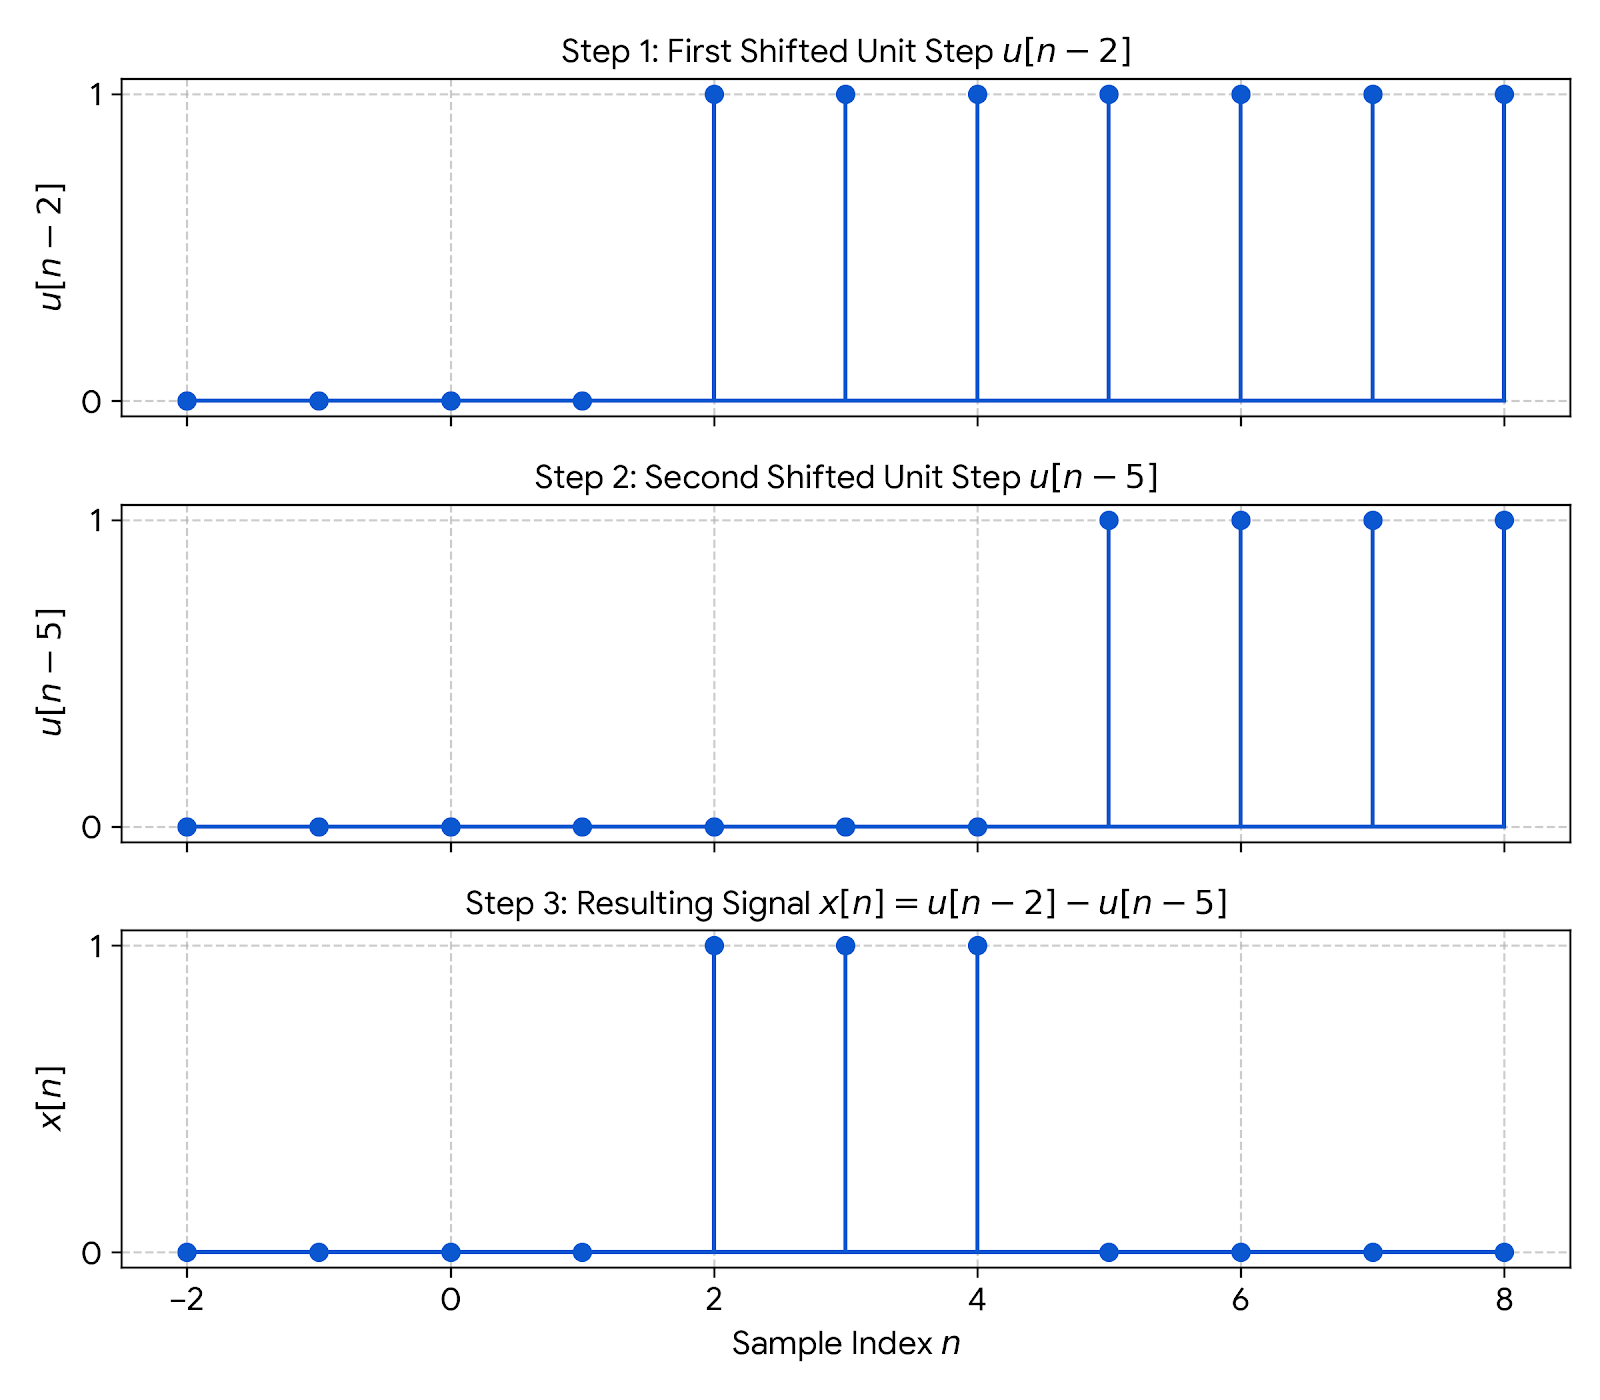
\includegraphics[keepaspectratio,alt={signal\_visualization.png}]{signal_visualization.png}}
\caption{signal\_visualization.png}
\end{figure}

\subsubsection{3. Classification of discrete-time
signals}\label{classification-of-discrete-time-signals}

\paragraph{3.1. Energy signals and power
signals}\label{energy-signals-and-power-signals}

\begin{itemize}
\tightlist
\item
  \textbf{Total Energy:}
\end{itemize}

\[  
E=\sum_{n=-\infty}^{\infty}|x[n]|^2  
\]

\begin{itemize}
\tightlist
\item
  \textbf{Average Power:}
\end{itemize}

\[  
P=\lim_{N\to\infty}  
\frac{1}{2N+1}  
\sum_{n=-N}^{N}|x[n]|^2  
\]

\begin{itemize}
\tightlist
\item
  An \textbf{energy signal} has a \textbf{finite, non-zero total energy}
  (\(0 < E < \infty\)), which forces its average power to be
  \textbf{zero} (\(P = 0\)).
\item
  A \textbf{power signal} has a \textbf{finite, non-zero average power}
  (\(0 < P < \infty\)), which means its total energy is
  \textbf{infinite} (\(E = \infty\)).
\item
  Signals that grow infinitely over time are neither energy nor power
  signals (\(E = \infty, P = \infty\)).
\end{itemize}

\emph{Example:}

\begin{itemize}
\tightlist
\item
  Unit Sample Signal \(\delta[n]\):

  \begin{itemize}
  \tightlist
  \item
    \textbf{Total Energy (\(E\)):}
    \[E = \sum_{n=-\infty}^{\infty} \vert{}\delta[n]\vert{}^2 = \vert{}\delta[0]\vert{}^2 = 1^2 = 1\]
  \item
    \textbf{Average Power (\(P\)):}
    \[P = \lim_{N\to\infty} \frac{1}{2N+1} \sum_{n=-N}^{N} \vert{}\delta[n]\vert{}^2 = \lim_{N\to\infty} \frac{1}{2N+1} (1) = 0\]
    Since \(0 < E < \infty\) and \(P = 0\), \textbf{\(\delta[n]\) is an
    energy signal}.
  \end{itemize}
\item
  Unit Step Signal \(u[n]\):

  \begin{itemize}
  \item
    \textbf{Total Energy (\(E\)):}

    \[E = \sum_{n=-\infty}^{\infty} \vert{}u[n]\vert{}^2 = \sum_{n=0}^{\infty} 1^2 = 1 + 1 + 1 + \dots = +\infty\]

    Because energy is infinite, \(u[n]\) cannot be an energy signal.
  \item
    \textbf{Average Power (\(P\)):}

    In the interval \([-N, N]\), the signal is \(1\) only for
    \(n = 0, 1, 2, \dots, N\) (which contains \(N + 1\) active samples):

    \[P = \lim_{N\to\infty} \frac{1}{2N+1} \sum_{n=0}^{N} 1 = \lim_{N\to\infty} \frac{N+1}{2N+1}\]

    Dividing numerator and denominator by \(N\):

    \[P = \lim_{N\to\infty} \frac{1 + 1/N}{2 + 1/N} = \frac{1 + 0}{2 + 0} = \frac{1}{2}\]

    Since \(0 < P < \infty\), \textbf{\(u[n]\) is a power signal}.
  \end{itemize}
\end{itemize}

\paragraph{3.2. Periodic signals and aperiodic
signals}\label{periodic-signals-and-aperiodic-signals}

\begin{itemize}
\tightlist
\item
  A signal \(x[n]\) is periodic if there exists a positive integer
  fundamental period \(N \in \mathbb{Z}^+\) such that
  \(x[n + N] = x[n]\) for all integer indices \(n\).
\item
  The smallest positive integer \(N\) satisfying this condition is
  called the \textbf{fundamental period}.
\item
  If no such integer \(N\) exists, the signal is aperiodic.
\item
  All periodic signals with non-zero values over an infinite duration
  are \textbf{power signals}.
\item
  For discrete complex exponentials \(x[n] = e^{j\omega_0 n}\) or
  sinusoids \(x[n] = \cos(\omega_0 n)\), periodicity requires that
  \(\frac{\omega_0}{2\pi} = \frac{k}{N}\) (a rational ratio), where the
  fundamental period is \(N = \frac{2\pi k}{\omega_0}\).
\end{itemize}

\paragraph{3.3. Symmetric (even) and antisymmetric (odd)
signals}\label{symmetric-even-and-antisymmetric-odd-signals}

\begin{itemize}
\tightlist
\item
  A signal is \textbf{even (symmetric)} if \(x[-n] = x[n]\) for all
  \(n\) (reflection across the vertical axis \(n = 0\)).
\item
  A signal is \textbf{odd (antisymmetric)} if \(x[-n] = -x[n]\) for all
  \(n\) (forces \(x[0] = 0\)).
\item
  \textbf{Decomposition:} Any arbitrary discrete-time signal \(x[n]\)
  can be uniquely split into a sum of its even part \(x_e[n]\) and odd
  part \(x_o[n]\): \[x[n] = x_e[n] + x_o[n]\] where:
  \[x_e[n] = \frac{1}{2}(x[n] + x[-n])\]
  \[x_o[n] = \frac{1}{2}(x[n] - x[-n])\]
\end{itemize}

\subsubsection{4. Simple Manipulations of Discrete-Time
Signals}\label{simple-manipulations-of-discrete-time-signals}

\paragraph{4.1. Time Shifting \& Time
Reversal}\label{time-shifting-time-reversal}

\[
x[\pm n \pm a], a \in \mathbb{N}
\]

\begin{itemize}
\tightlist
\item
  \textbf{Time Shifting (\(x[n \pm a]\)):} Moving the signal along the
  time axis without changing its shape.

  \begin{itemize}
  \tightlist
  \item
    \(x[n - a]\) delays (shifts right) the signal by \(a\) units.
  \item
    \(x[n + a]\) advances (shifts left) the signal by \(a\) units.
  \end{itemize}
\item
  \textbf{Time Reversal / Folding (\(x[-n]\)):} Reflects the signal
  about \(n = 0\).
\item
  \textbf{Combined Shift \& Reversal (\(x[-n \pm a]\)):} Order of
  operations matters:

  \begin{itemize}
  \tightlist
  \item
    First shift \(x[n]\) to get \(x[n \pm a]\), then reverse time
    \(n \to -n\) to get \(x[-n \pm a]\).
  \item
    Alternatively, factor as \(x[-(n \mp a)]\): first fold
    \(x[n] \to x[-n]\), then shift in the direction dictated by the
    factored sign.
  \end{itemize}
\end{itemize}

\paragraph{4.2. Up-sampling \&
Down-sampling}\label{up-sampling-down-sampling}

\[
x[cn], c \in \mathbb{N}
\]

\begin{itemize}
\tightlist
\item
  \textbf{Down-sampling / Decimation
  (\(x[cn], c \in \mathbb{N}, c > 1\)):}

  \begin{itemize}
  \tightlist
  \item
    Keeps every \(c\)-th sample and discards the rest (\(c-1\) samples
    dropped between kept samples).
  \item
    Shrinks/compresses the signal in time domain and leads to spectrum
    expansion in frequency domain (potential aliasing if not
    pre-filtered).
  \end{itemize}
\item
  \textbf{Up-sampling / Interpolation (\(c \in \mathbb{N}, c > 1\)):}

  \begin{itemize}
  \tightlist
  \item
    Expressed as
    \(x_u[n] = \begin{cases} x[n/c], & \text{if } n \text{ is a multiple of } c \\ 0, & \text{otherwise} \end{cases}\)
  \item
    Inserts \(c - 1\) zero-valued samples between consecutive original
    samples, expanding the signal in the time domain.
  \end{itemize}
\end{itemize}

\subsection{III. Discrete-Time
Systems}\label{iii.-discrete-time-systems}

\subsubsection{1. Representations}\label{representations-1}

\paragraph{1.1. Input-Output Description of
Systems}\label{input-output-description-of-systems}

\begin{itemize}
\tightlist
\item
  A discrete-time system operates on an input sequence \(x[n]\) to
  produce an output sequence \(y[n]\), represented as
  \(y[n] = \mathcal{T}\{x[n]\}\).
\item
  Systems are represented by difference equations: Linear
  constant-coefficient difference equations (LCCDE) relate the current
  output to past outputs and current/past inputs:
  \[\sum_{k=0}^{N} a_k y[n-k] = \sum_{m=0}^{M} b_m x[n-m]\]
\end{itemize}

\paragraph{1.2. Block Diagram Representation of Discrete-Time
Systems}\label{block-diagram-representation-of-discrete-time-systems}

\begin{itemize}
\tightlist
\item
  Constructed using three basic functional building blocks:

  \begin{itemize}
  \tightlist
  \item
    \textbf{Adder:} Adds two signals, \(y[n] = x_1[n] + x_2[n]\).
  \item
    \textbf{Constant Multiplier (Gain):} Scales a signal by a constant,
    \(y[n] = a \cdot x[n]\).
  \item
    \textbf{Unit Delay Element (\(z^{-1}\)):} Delays a signal by one
    sample, \(y[n] = x[n-1]\). (A unit advance \(z\) yields \(x[n+1]\)).
  \end{itemize}
\end{itemize}

\subsubsection{2. Classification of Discrete-Time
Systems}\label{classification-of-discrete-time-systems}

\paragraph{2.1. Static vs dynamic
systems}\label{static-vs-dynamic-systems}

\begin{itemize}
\tightlist
\item
  \textbf{Static (Memoryless):} The output \(y[n]\) at index \(n\)
  depends \emph{only} on the input \(x[n]\) at that same index \(n\)
  (e.g., \(y[n] = C x^2[n]\)).
\item
  \textbf{Dynamic (With Memory):} The output \(y[n]\) depends on past or
  future values of the input or output (e.g., \(y[n] = x[n] + x[n-1]\)).
\end{itemize}

\paragraph{2.2. Time-invariant vs time-variant
systems}\label{time-invariant-vs-time-variant-systems}

\begin{itemize}
\tightlist
\item
  \textbf{Time-Invariant (Shift-Invariant):} A time shift in the input
  causes an identical time shift in the output: if
  \(\mathcal{T}\{x[n]\} = y[n]\), then
  \(\mathcal{T}\{x[n-k]\} = y[n-k]\) for all integer \(k\).
\item
  \textbf{Time-Variant:} The system's input-output relationship changes
  over time (e.g., coefficients depend on \(n\), as in
  \(y[n] = n \cdot x[n]\), or time operations occur, as in
  \(y[n] = x[-n]\)).
\end{itemize}

\paragraph{2.3. Linear vs nonlinear
systems}\label{linear-vs-nonlinear-systems}

\begin{itemize}
\tightlist
\item
  \textbf{Linear:} Satisfies the principle of \textbf{superposition}
  (both additivity and homogeneity):
  \[\mathcal{T}\{a \cdot x_1[n] + b \cdot x_2[n]\} = a \cdot \mathcal{T}\{x_1[n]\} + b \cdot \mathcal{T}\{x_2[n]\}\]
\item
  \textbf{Nonlinear:} Fails superposition (e.g., contains powers, square
  roots, absolute values, or non-zero initial conditions like
  \(y[n] = x^2[n]\) or \(y[n] = x[n] + 3\)).
\end{itemize}

\paragraph{2.4. Causal vs non-causal
systems}\label{causal-vs-non-causal-systems}

\begin{itemize}
\tightlist
\item
  \textbf{Causal:} The output \(y[n]\) at any index \(n\) depends
  \emph{only} on present and/or past inputs \(x[k]\) (\(k \le n\)). It
  cannot depend on future inputs.
\item
  \textbf{Non-Causal:} The output \(y[n]\) depends on future input
  samples \(x[k]\) (\(k > n\)) (e.g., \(y[n] = x[n+1]\)). Non-causal
  systems cannot be implemented in real time, but can process
  pre-recorded data.
\end{itemize}

\paragraph{2.5. Stable vs unstable
systems}\label{stable-vs-unstable-systems}

\begin{itemize}
\tightlist
\item
  \textbf{BIBO Stable (Bounded-Input, Bounded-Output):} Every bounded
  input \(|x[n]| \le M_x < \infty\) produces a bounded output
  \(|y[n]| \le M_y < \infty\).
\item
  \textbf{LTI System Stability Condition:} An LTI system with impulse
  response \(h[n]\) is BIBO stable if and only if its impulse response
  is \textbf{absolutely summable}:
  \[\sum_{n=-\infty}^{\infty} |h[n]| < \infty\]
\end{itemize}

\emph{Next session:} Analysis of Discrete-Time Linear Time-Invariant
Systems
